\section{Hardware Platform}
\label{sec:back:hw}

This project targets the EFM32GG \gls{mcu} developed by Silicon Labs.
The following sections presents the EFM32 family of microcontrollers and a couple of development kits that utilize the Giant Gecko \gls{mcu}, soldered with a handful of different peripherals.

\subsection{EFM32}
\label{sub:emf32}
\todo{There's some rough edges of the language in this section. Needs to be rephrased}

ARM Cortex-M is a family of 32-bit RISC processor cores, intended to be used by applications that require low cost and energy-usage.
These factors are crucial in modern systems and applications where energy efficiency is of great importance.
For example with the \gls{iot} \cite{Valhouli2010}, where we predict a future where tens of billions of devices will be connected to the Internet, ranging from Super Computers down to small embedded devices that might be used to power up and control everything from cars to light bulbs via the Internet.
The different processor cores of the Cortex-M family are summarized in \autoref{tab:cortex_m}.

\begin{table}[h]
\begin{center}
\begin{tabular}{r|l}
    \textbf{Name} & \textbf{Target features}            \\
    \hline
    Cortex-M0 & Lowest cost and lowest area              \\
    Cortex-M0+ & Lowest power                            \\
    Cortex-M1 & Designed for implementation in FPGAs     \\
    Cortex-M3 & Performance efficiency                   \\
    Cortex-M4 & DSP, SIMD, FP                            \\
    Cortex-M7 & Cache, TCM, AXI, ECC, double + single FP \\
    \hline
    \end{tabular}
\end{center}
\caption{Cortex-M family of processor cores}
\label{tab:cortex_m}
\end{table}

\todo{Include the table with flash size instead?}
The EFM32 family of microcontrollers are all based on different Cortex-M processors, some of their features are summarized in \autoref{tab:efm32_family}.
The focus of these microcontrollers is energy efficiency and low power-consumption in resource-constraint environments.
The EFM32GG, usually referred to with the name \chip{Giant Gecko}, is a versatile chip that is in the upper end in the Cortex-M series.
This is the processor core that is targeted in this project, and for the sake of simplicity we will refer to this chip as the {\gecko}.

The microcontrollers implement several different methods for reducing the power consumption.
The most important way to achieve low power consumption is by turning off the different parts of the chip that are inactive, so that these parts do no longer draw any power from the overall system.
The EFM32 processors features five different energy modes, or sleep modes, ranging from EM0 (Energy Mode 0) where the core is on, to EM4 where the processor can only wake up on specific interrupt signals.
The different peripherals provided with the EFM32's operate in different energy modes.
This system allows applications to utilize many different peripherals for data collection, while the processor itself is turned off.
The peripherals then has the opportunity to wake up the processor on different interrupt-signals and transfer data to it, in order to do general processing.

\begin{table}[b]
\begin{center}
    \begin{tabular}{r|l|l}
    \textbf{Name} & \textbf{Processor} & \textbf{Speed (MHz)} \\
    \hline
    Zero Gecko    & ARM Cortex-M0+ & 24 \\
    Tiny Gecko    & ARM Cortex-M3  & 32 \\
    Gecko         & ARM Cortex-M3  & 32 \\
    Leopard Gecko & ARM Cortex-M3  & 48 \\
    Giant Gecko   & ARM Cortex-M3  & 48 \\
    Wonder Gecko  & ARM Cortex-M4  & 48 \\
    \hline
    \end{tabular}
\end{center}
\caption{EFM32 Product Family \cite{web:silabs}}
\label{tab:efm32_family}
\end{table}

% \begin{table}[H]
%   \centering
%   \begin{tabular}{|l|l|l|l|l|}
%     \hline
%     Family & Core & Speed (MHz) & Flash Memory (kB) & RAM (kB) \\
%     \hline
%     Zero Gecko & ARM Cortex-M0+ & 24 & 4, 8, 16, 32 & 2, 4 \\
%     Tiny Gecko & ARM Cortex-M3 & 32 & 4, 8, 16, 32 & 2, 4 \\
%     Gecko & ARM Cortex-M3 & 32 & 16, 32, 64, 128 & 8, 16 \\
%     Leopard Gecko & ARM Cortex-M3 & 48 & 64, 128, 256 & 32 \\
%     Giant Gecko & ARM Cortex-M3 & 48 & 512, 1024 & 128 \\
%     Wonder Gecko & ARM Cortex-M4 & 48 & 64, 128, 256 & 32 \\
%     \hline
%   \end{tabular}
%   \caption{EFM32 Product Family \cite{web:silabs}}
%   \label{tab:efm32-family}
% \end{table}

\subsection{Evaluation boards}

Silicon Labs provides a wide range of development-kits and -boards that are targeted for general development and testing of applications based on the EFM32's.
Two of these boards are available with the {\gecko} and we have used both of them in this project.
The simplest of the two are the \chip{Giant Gecko} Starter Kit, which is depicted in \autoref{fig:efm32gg-stk3700}.
This board contains a few LEDs and buttons, a couple of sensors to demonstrate a wide range of use-cases, and a segment LCD display.
It also includes an expansion header that can be used to connect with third party devices and peripherals, and a JLink debug interface over USB.

\begin{figure}[H]
  \begin{center}
    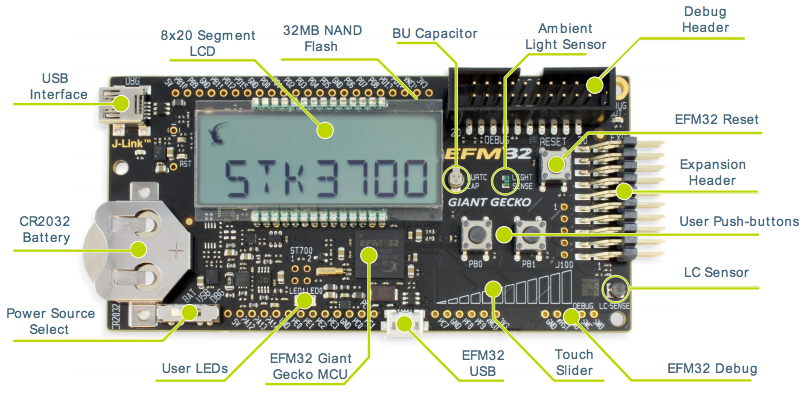
\includegraphics[scale=0.4]{figures/efm32gg-stk3700}
  \end{center}
  \caption{The Giant Gecko Starter Kit - EFM32GG-STK3700 \cite{UM-STK} }
  \label{fig:efm32gg-stk3700}
\end{figure}

As seen in \autoref{fig:efm32gg-dk3750} the Giant Gecko Development Kit is a more complex board.
It features a TFT touch Display, a prototyping board which exposes all the \gls{mcu} pins on headers.
The \gls{mcu} itself is also soldered on a pluggable board, which makes the development kit a suitable system for testing a wide range of different applications.
We have also used the Biometrix-EXP Evaluation board, which features a handful of additional sensors, in addition to the two board mentioned already.
The Biometrix-EXP Evaluation board is shown in \autoref{fig:biometric-exp} and connects directly with the Expansion Header available on the Starter Kit.

\begin{figure}[H]
  \begin{center}
    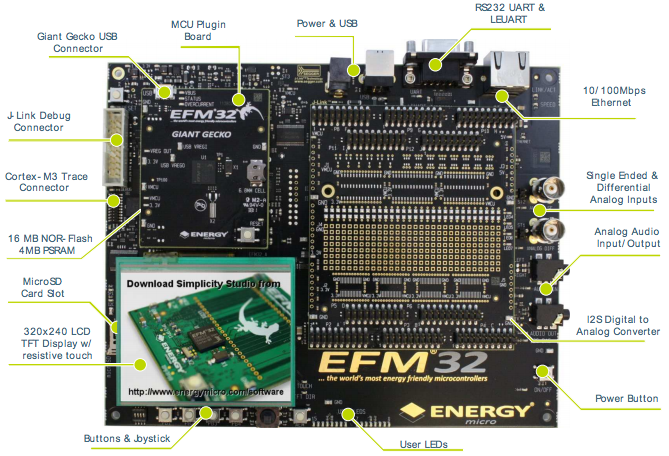
\includegraphics[scale=0.5]{figures/efm32gg-dk3750}
  \end{center}
  \caption{The Giant Gecko Development Kit - EFM32GG-DK3750 \cite{UM-DK}}
  \label{fig:efm32gg-dk3750}
\end{figure}

\begin{figure}[H]
  \begin{center}
    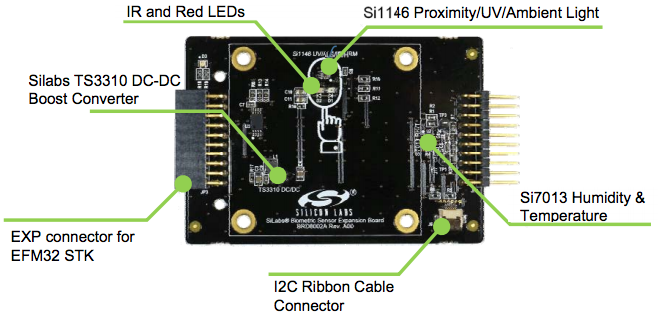
\includegraphics[scale=0.5]{figures/biometric-exp}
  \end{center}
  \caption{The Biometric-EXP Evaluation Board - BIOMETRIC-EXP-EVB \cite{UG-BIO-EXP}}
  \label{fig:biometric-exp}
\end{figure}


\autoref{tab:hw:boards} summarizes the different hardware devices that are referred to throughout this report.
The original device-names are shortened in order to simplify reading.

\begin{table}[H]
  \begin{tabular}{l|l|l}
    \textbf{Product Name} & \textbf{Description} & \textbf{Short name} \\
    \hline
    EFM32GG & The Giant Gecko Microcontroller & \texttt{Gecko} \\
    EFM32GG-STK3700 & Giant Gecko Starter Kit & \texttt{STK} \\
    EFM32GG-DK3750 & Giant Gecko Development Kit & \texttt{DK} \\
    BIOMETRIC-EXP-EVB & Biometric Sensor Expansion Board & \texttt{BIO-EXP} \\
    \hline
  \end{tabular}
  \caption{Hardware devices}
  \label{tab:hw:boards}
\end{table}

\subsubsection{Peripherals}
\label{sub:peripherals}
\todo{This subsection might not be relevant. Do we want a subsection to describe the peripherals of the GG with a little more detail?}

In this project we have only focused on writing software for the Giant Gecko series of microcontrollers.
We have utilized two different development boards that both features the EFM32GG990 microcontroller,
thus we have limited implementation of bindings to only support a handful of peripherals that are
available with this device. A block diagram of the device and its peripherals are shown in
\autoref{fig:efm32gg990_block_diagram}.

\begin{figure}[b]
\centering
\missingfigure{EFM32GG990 block diagram}
\caption{Some caption}
\label{fig:efm32gg990_block_diagram}
\end{figure}

For this project, the porting of library bindings are only interesting if the peripherals exposed by
the library are actually going to be used. The two boards we have access to implements many external
sensors and peripherals that are all controlled through \emlib. It is only interesting to write
bindings and abstractions for the core functionality of \emlib and the parts of the library that
lets us control peripherals that we use in throughout the projects.
